\documentclass[aspectratio=169]{beamer}

\usetheme[font=noto,summary]{UiO}

\usepackage[utf8]{inputenc}
\usepackage{babel}

\usepackage[backend=biber,style=authoryear,maxcitenames=2]{biblatex}
\addbibresource{Library.bib}

\usepackage{graphicx}
\usepackage{booktabs}
\usepackage{hyperref}

\title[Protocol Racing]{Protocol Racing}
\subtitle{Is it really an advancement?}
\author[Joar Heimonen]{Joar Heimonen}
\date{\today}
\uioemail{contact@joar.me}

\begin{document}

\uiofrontpage[dept={}, image={image.png}, inverted]

\begin{frame}{Agenda}
  \tableofcontents
\end{frame}

\section{A bit of history}
\begin{frame}{IPv4}
  \begin{itemize}
    \item \textbf{RFC 791} – \emph{Internet Protocol}
    \item Written for DARPA in 1981 (before the IETF existed)
    \item Designed to interconnect different packet-switched networks (ARPANET, SATNET, university nets)
    \item Created under the assumption that every device would have its own globally unique, routable address
    \item 32-bit address space — \(2^{32} = 4{,}294{,}967{,}296\) possible addresses
    \item Sounds like a lot\ldots\ until you remember that there are 8 billion people alive
  \end{itemize}
\end{frame}

\begin{frame}{The problem with IPv4}
  \centering
  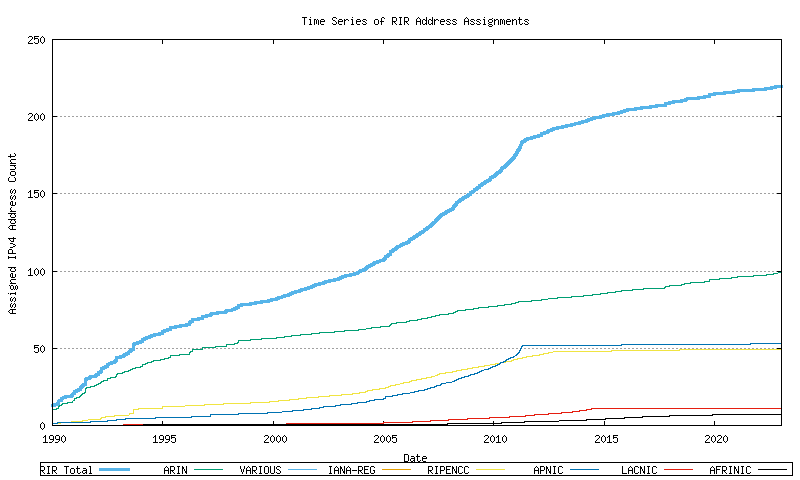
\includegraphics[width=0.8\textwidth]{fig09.png}
  \\
  {\tiny Source: \parencite{IPv4AddressReport}}
\end{frame}

\section{Main}
\begin{frame}{Key Idea}
  \begin{block}{Takeaway}
    Keep each slide focused on one idea.
  \end{block}
\end{frame}

\section{Wrap-up}
\begin{frame}
  \centering
  \vfill
  {\usebeamerfont{title}\usebeamercolor[fg]{title}\LARGE Questions?}
  \vfill
\end{frame}

\begin{frame}[allowframebreaks]{References}
  \printbibliography
\end{frame}
\end{document}
